\documentclass{beamer}
\usetheme{Warsaw}

\usepackage{hyperref}
\usepackage{tikz}
\usepackage{varwidth}
\usetikzlibrary{arrows,shapes}
\usepackage{amsmath}
\usepackage{algorithm}
%\usepackage{algpseudocode}

\usepackage{graphicx}
\graphicspath{{images/}}

\title[Assignment 1 \hspace{3.5cm} Page \insertframenumber]{\textsc{Assignment 1}}
\subtitle{}

\institute{\textit{prepared by}\\ Mohamed Saleh, 1111113245, 0163698424\\
Loie Hesham , 1091105774, 0102691266 \\[0.3cm] \textsc{Faculty of Computing \& Informatics \\ Multimedia University\\ Cyberjaya, Malaysia} \\ 
\includegraphics[scale=0.5]{mmulogo}}


\date{}

\begin{document}

%------------------- Slide ------------------------------

\begin{frame}
\titlepage
\end{frame}

%------------------- Slide ------------------------------
\begin{frame}
\frametitle{}
\framesubtitle{}
{\Large {\bf Wireless Face Interface: Using voluntary gaze direction and facial muscle activations
for human–computer interaction } }

Outi Tuisku, Veikko Surakka, Toni Vanhala , Ville Rantanen, Jukka Lekkala 
\end{frame}
%------------------- Slide ------------------------------


\begin{frame}
\frametitle{Introduction}
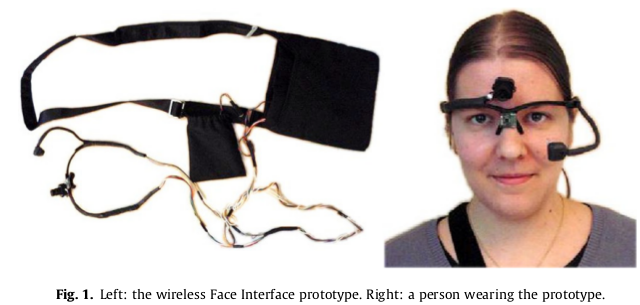
\includegraphics[scale=0.4]{1.png}
 \begin{itemize}
\item  whats the main aim of this article?  
\item  what is the face interface device?
\item  how does it work?`
\end{itemize}
\framesubtitle{}

\end{frame}

%------------------- Slide ------------------------------
\begin{frame}
\frametitle{Motivation and Context}
 \begin{itemize}
\item continuing the earlier researches and studies in the field .
\item To test and evaluate the different methods selecting . 
\item The benefits of such device . 
\end{itemize}
\framesubtitle{}

\end{frame}

%------------------- Slide ------------------------------
\begin{frame}
\frametitle{Research Questions}
\framesubtitle{}
\begin{itemize}
\item To find which one is better between the two selection technique (frowning or the raising eyebrows)?
\item How the device will preform on a wider variety of tasks?
\end{itemize} 
\end{frame}

%------------------- Slide ------------------------------
\begin{frame}
\frametitle{Critical Literature Review}
\framesubtitle{}
\begin{itemize}
\item Earlier studies of Surakka 2004,2005 \\
- Used remote eye tracker and EMG amplifier	
\item Chin et al. (2008) \\
- Used the facial EMG to correct the inaccuracy of the eye tracker
\item Fitts’ law \\
- difficulty of a pointing task (ID) \\
- the movement time (MT)\\
- index of performance (IP) 
\item Subjective ratings \\
- Used to rate the participants experience
 
\end{itemize}

\end{frame}

%------------------- Slide ------------------------------
\begin{frame}
\frametitle{Research Method and Results}
\framesubtitle{}

\begin{itemize}
\item 20 voluntary participants
\item range 19–43 years
\item All participants had normal vision
\item Samsung SyncMaster 24" widescreen 
\item viewing distance of 60 cm
\item Windows XP operating system

\end{itemize}

\end{frame}

%------------------- Slide ------------------------------

\begin{frame}
\frametitle{Research Method and Results }

%\includegraphics[scale=0.8]{}
\begin{itemize}
\item home square and a target circle on the screen
\item select the home square first, then the target circle
\item A pause of 2000 ms
\item The width of the home square = 30mm

\end{itemize}

\end{frame}

%------------------- Slide ------------------------------

\begin{frame}
\frametitle{Research Method and Results }
%\includegraphics[scale=0.35]{.png}
\begin{itemize}
\item the participants were introduced to the equipment
\item practice before the actual experiment = 5 min.
\item short relaxation period 
\item The scale varied from -4 to +4

\end{itemize}


\end{frame}

%------------------- Slide ------------------------------


\begin{frame}
\frametitle{Research Method and Results }
\framesubtitle{}
%\includegraphics[scale=0.3]{.png}
\begin{itemize}
\item Mixed-model analyses of variance(ANOVA)
\item Bonferroni corrected {\it t}-tests to detect the target circle clicking error 
\item 40 mm diameter, faster
\item The raising technique, faster pointing task times
\item frownig technique, higher mean error rate
\item  Fitts' law was performed on, distances from 60 mm to 260 mm 
\end{itemize}
\end{frame}


%------------------- Slide ------------------------------
\begin{frame}
\frametitle{Conclusion }
\framesubtitle{}
We Conclude that: 
\begin{itemize} 
\item the wireless face interface device is that use the gaze direction to point and the facial muscle movement (Frowning or Rising eyebrows) to select objects on the PC screen .
\item Differences between frowning and rising the eyebrows .
\item Whats the improvements and differences between the device and the earlier devices. 
\item The device's potentials in the future .
\end{itemize} 
\end{frame}

%------------------- Slide ------------------------------
\begin{frame}
\frametitle{Q and A}

\Huge Questions And Answers
\framesubtitle{}

\end{frame}

\end{document}